\section{Evaluation}
\label{remy:eval}

We used ns-2 to evaluate the algorithms generated by Remy and compare
them with several other congestion-control methods, including both
end-to-end schemes and schemes with router assistance. This section
describes the network and workload scenarios and our findings.

\subsection{Simulation setup and metrics}

\noindent {\bf Congestion-control protocols.} The end-to-end schemes
we compared with are NewReno, Vegas, Cubic, and Compound. In addition,
we compared against two schemes that depend on router assistance: XCP,
and Cubic over stochastic fair queueing~\cite{sfq} with each queue
running CoDel~\cite{CoDel}. We use Nichols's published sfqCoDel
implementation (version released in March 2013) for
ns-2.\footnote{\url{http://www.pollere.net/Txtdocs/sfqcodel.cc}} The
Cubic, Compound, and Vegas codes are from the Linux implementations
ported to ns-2 and available in ns-2.35.  For the datacenter
simulation, we also compare with the DCTCP ns-2.35
patch.\footnote{\url{http://www.stanford.edu/~alizade/Site/DCTCP.html}}

{\bf RemyCCs.} We used Remy to construct three general-purpose
RemyCCs. Each one was designed for an uncertain network model with the
dumbbell topology of Figure~\ref{fig:dumbbell}, but with three
different values of $\delta$ (the relative importance of delay): 0.1,
1, and 10. The parameters of the network and traffic model used at
design time were:

\vspace{\baselineskip}

\begin{tabular}{lll}
\bf Quantity & \bf Design range & \bf Distribution \\
\hline $n$ max senders & 1--16 & uniform \\
``on'' process & mean 5~s & exponential \\
``off'' process & mean 5~s & exponential \\
link speed & 10--20~Mbps & uniform \\
round-trip time & 100--200~ms & uniform \\
queue capacity & unlimited & \\
\end{tabular}

\vspace{\baselineskip}

The model captures a 64-fold range of bandwidth-delay product per
user. Each RemyCC took about 3--5 CPU-days to optimize. Calculations
were run on Amazon EC2 and on an 80-core and 48-core server at MIT. In
wall-clock time, each RemyCC took a few hours to be constructed.
The RemyCCs contain between 162 and 204 rules each.

We also used Remy to assess how performance varies based on the
specificity of the assumptions used at design time, by building
one RemyCC for a link speed known exactly \emph{a priori}, and
one that assumes only that the link speed will lie within a tenfold range:

\vspace{\baselineskip}

\begin{tabular}{lll}
\bf Quantity & \bf Design range & \bf Distribution \\
\hline $n$ max senders & 2 & uniform \\
``on'' process & mean 5~sec & exponential \\
``off'' process & mean 5~sec & exponential \\
link speed & 15~Mbps (``$1\times$'') & exact \\
link speed & 4.7--47~Mbps (``$10\times$'') & uniform \\
round-trip time & 150~ms & exact \\
queue capacity & unlimited & \\
\end{tabular}

\vspace{\baselineskip}

In most experiments, all the sources run the same protocol; in some,
we pick different protocols for different sources to investigate how
well they co-exist. Each simulation run is generally 100 seconds long,
with each scenario run at least 128 times to collect summary
statistics.

\begin{figure}
%\vspace{\baselineskip}
\begin{centering}
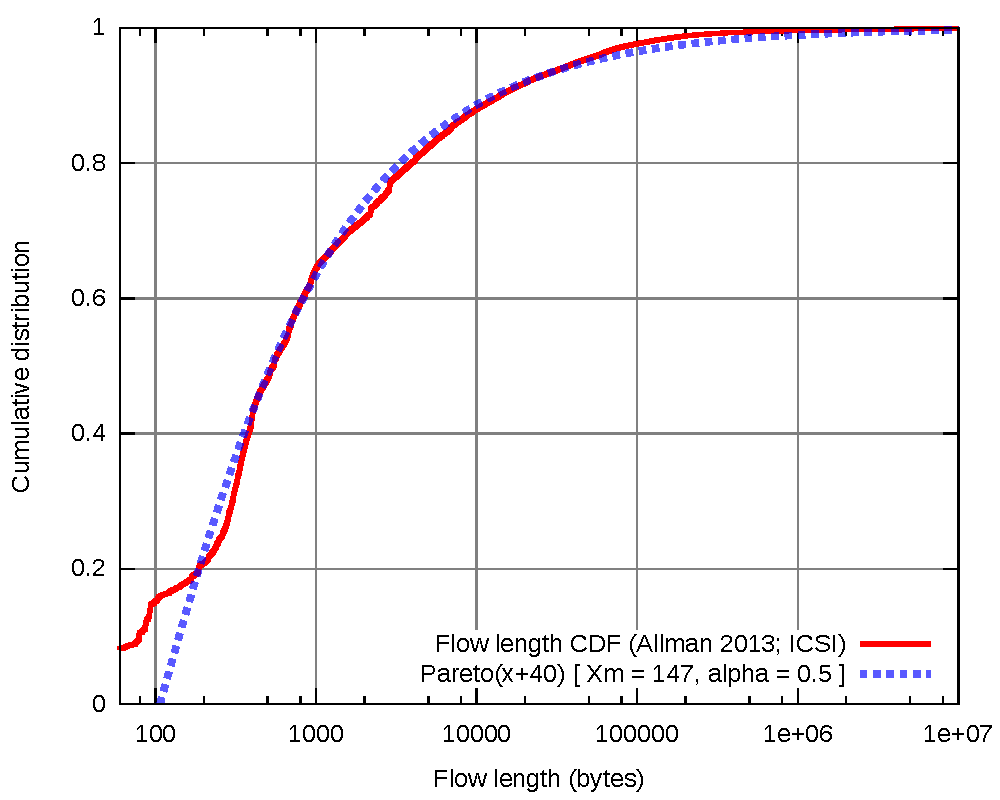
\includegraphics[width=\columnwidth]{flowlength.pdf}
\end{centering}
\caption{Observed Internet flow length distribution matches a Pareto ($\alpha = 0.5$)
distribution, suggesting mean is not well-defined.}
\label{f:flowcdf}
\end{figure}

\medskip
\noindent
{\bf Workloads.} Each source is either ``on'' or ``off'' at any point
in time. In the evaluation, we modeled the ``off'' times as exponentially distributed, and
the ``on'' distribution in one of three different ways:
\begin{itemize}
\item {\em by time}, where the source sends as many bytes as the
  congestion-control protocol allows, for a duration of time picked
  from an exponential distribution,
\item {\em by bytes}, where the connection sends as many bytes as
  given by an exponential distribution of a given average and shape,
  and
\item {\em by empirical distribution}, using the flow-length CDF from
  a large trace captured in March 2012 and published
  recently~\cite{allman-ccr-trace}. The flow-length CDF matches a
  Pareto distribution with the parameters given in
  Figure~\ref{f:flowcdf}, suggesting that the underlying distribution
  does not have finite mean. In our evaluation, we add 16 kilobytes to
  each sampled value to ensure that the network is loaded.
\end{itemize}

\medskip
\noindent {\bf Topologies.} We used these topologies in our experiments:
\begin{enumerate}
\item {\bf Single bottleneck (``dumbbell''):} The situation in
  Figure~\ref{fig:dumbbell}, with a 1,000-packet buffer, as might be
  seen in a shared cable-modem uplink. We tested a configuration whose
  link speed and delay were within the RemyCC design ranges:

%\vspace{\baselineskip}

\begin{tabular}{lll}
\bf Quantity & \bf Range & \bf Distribution \\
\hline link speed & 15~Mbps & exact \\
round-trip time & 150~ms & exact \\
queue capacity & 1000 pkts (tail drop) \\
\end{tabular}

\item {\bf Cellular wireless:} We measured the downlink capacity of the
  Verizon and AT\&T LTE cellular services while mobile, by carefully
  saturating the downlink (without causing buffer overflow) and
  recording when packets made it to the user device. We recreate this
  link within ns-2, queueing packets until they are released to the
  receiver at the same time they were released in the trace. This
  setup probes the RemyCC's resilience to ``model mismatch'' --- in
  both the Verizon and AT\&T traces, throughput and round-trip time
  were outside the limits of the RemyCC design range.
  
%\vspace{\baselineskip}

\begin{tabular}{lll}
\bf Quantity & \bf Range & \bf Distribution \\
\hline link speed & varied 0--50~Mbps & empirical \\
round-trip time & 50~ms & exact \\
queue capacity & 1000 pkts (tail drop) \\
\end{tabular}

\item {\bf Differing RTTs:} Cases where different RemyCCs, contending for
  the same link, had different RTTs to their corresponding
  receiver. We analyzed these cases for throughput and delay fairness
  and compared with existing congestion-control schemes.

\begin{tabular}{lll}
\bf Quantity & \bf Range & \bf Distribution \\
\hline $n$ max senders & 4 \\
``on'' process & $16 \times 10^3$--$3.3 \times 10^9$ bytes & Fig.~\ref{f:flowcdf}\\
``off'' process & mean 0.2~sec & exponential \\
link speed & 10~Mbps & exact \\
queue capacity & 1000 pkts (tail drop) \\
\end{tabular}

\item {\bf Datacenter:} We compared a RemyCC against
  DCTCP in a simulated datacenter topology.

\begin{tabular}{lll}
\bf Quantity & \bf Range & \bf Distribution \\
\hline $n$ max senders & 64 & exact \\
``on'' process & mean 20 megabytes & exponential \\
``off'' process & mean 0.1~sec & exponential \\
link speed & 10~Gbps & exact \\
round-trip time & 4~ms & exact \\
queue capacity & 1000 pkts (tail drop) & (for RemyCC) \\
queue capacity & modified RED & (for DCTCP) \\
\end{tabular}

\end{enumerate}

%In addition, we investigate:
%\begin{enumerate} 
%\item[5.] {\bf Competing protocols:} We assessed how a RemyCC ``played with''
%  existing congestion-control schemes (Cubic and Compound) when contending
%  for the same bottleneck link.
%\item [6.] {\bf Sensitivity of design range:} We investigated how
%  helpful prior knowledge of the network is to the performance of
%  Remy's generated algorithms.
%\end{enumerate}


\medskip
\noindent {\bf Metrics.}  We measure the throughput and average
queueing delay observed for each source-destination pair. With an
on-off source, measuring throughput takes some care.  We define the
throughput of a pair as follows. Suppose the pair is active during
(non-overlapping) time intervals of length $t_1, t_2, \ldots$ during
the entire simulation run of $T$ seconds. If in each interval the
protocol successfully receives $s_i$ bytes, we define the throughput
for this connection as $\sum s_i / \sum t_i$.%  Of course, this
%throughput cannot exceed the bottleneck link rate.

We are interested in the end-to-end delay as well; the reasoning
behind Remy's objective function and the $\delta$ parameter is that
protocols that fill up buffers to maximize throughput are not as
desirable as ones that achieve high throughput \emph{and} low delay
--- both for their effect on the user, who may prefer to get his
packets to the receiver sooner, as well as any other users who share
the same FIFO queue.

We present the results for the different protocols as {\bf
  throughput-delay plots}, where the log-scale $x$-axis is the
queueing delay (average per-packet delay in excess of minimum
RTT). Lower, better, delays are to the right.  The $y$-axis is the
throughput. Protocols on the top right are the best on such
plots. We take each individual 100-second run from a simulation as one
point, and then compute the 1-$\sigma$ elliptic contour
of the maximum-likelihood 2D Gaussian distribution that explains the
points. To summarize the whole scheme, we plot the median per-sender
throughput and queueing delay as a circle.

Ellipses that are narrower in the throughput or delay axis correspond
to protocols that are more consistent in allocating those
quantities. Protocols with large ellipses are those where
identically-positioned users differ widely in experience based on the
luck of the draw or the timing of their entry to the
network.\footnote{The ellipse represents the variability of the
  results among all nodes across all simulation runs. Thus, the notion
  of ``variability'' here includes both within-run variability or
  fairness (differing results among nodes that compete
  concurrently) as well as variability across runs. For the most part, our
  100-second simulation runs were long enough, relative to flow
  durations, that the ellipses can broadly be interpreted as
  an indicator of fairness.} The orientation of an ellipse
represents the {\em covariance between the throughput and delay}
measured for the protocol; if the throughput were uncorrelated with
the queueing delay (note that we show the queueing delay, not the
RTT), the ellipse's axes would be parallel to the graph's.  Because of
the variability and correlations between these quantities in practice,
we believe that such throughput-delay plots are an instructive way to
evaluate congestion-control protocols; they provide more information
than simply reporting mean throughput and delay values.

\subsection{Single-bottleneck results}

We start by investigating performance over the simple, classic
single-bottleneck ``dumbbell'' topology.  Although it does not model
the richness of real-world network paths, the dumbbell is a valuable
topology to investigate because in practice there are many
single-bottleneck paths experienced by Internet flows.

\begin{figure}
%\vspace{\baselineskip}
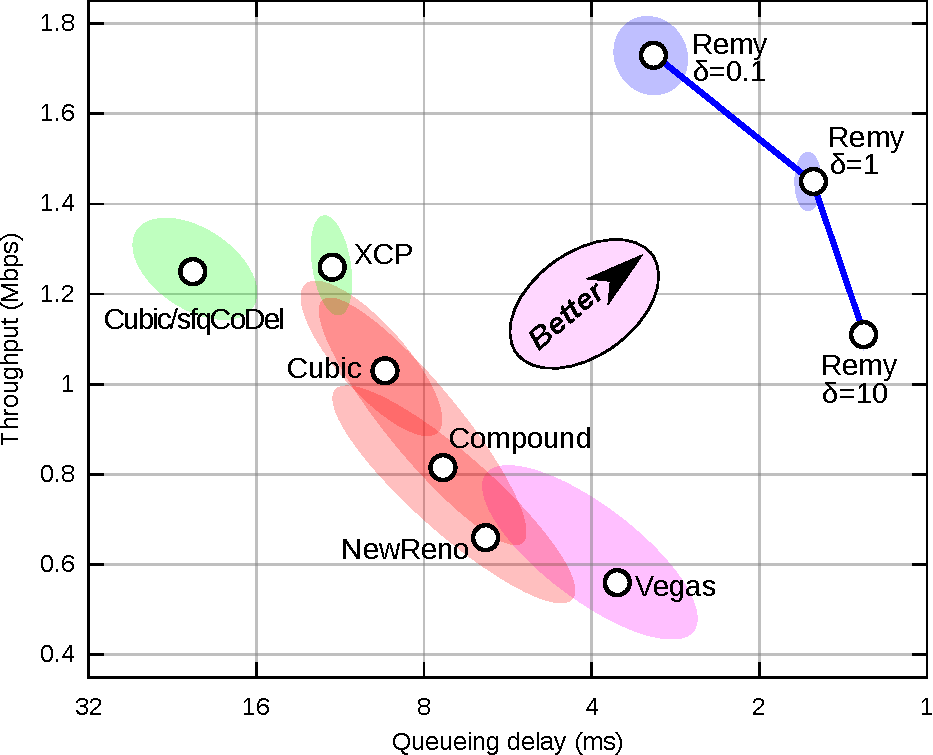
\includegraphics[width=\columnwidth]{eth8-final-bytes.pdf}
\caption{Results for each of the schemes over a 15~Mbps dumbbell
  topology with $n = 8$ senders, each alternating between flows of
  exponentially-distributed byte length (mean 100 kilobytes) and
  exponentially-distributed off time (mean 0.5 s). Medians and
  1-$\sigma$ ellipses are shown. The blue line represents the
  efficient frontier, which here is defined entirely by
  the RemyCCs.}

\label{f:tpdelaydb4}

\end{figure}

\begin{figure}
%\vspace{\baselineskip}
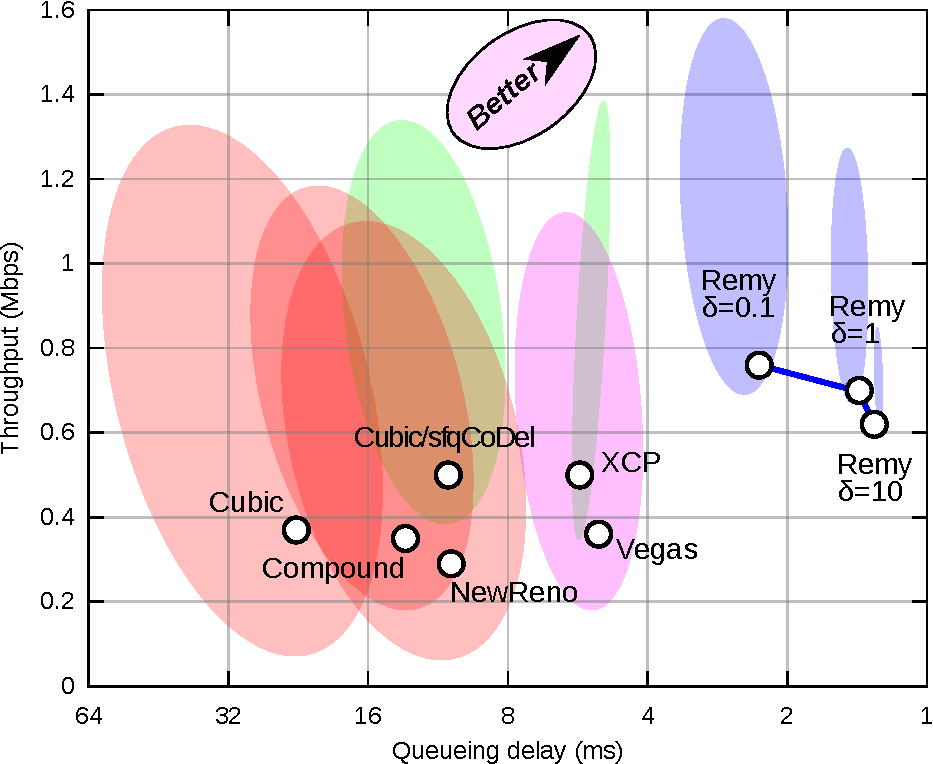
\includegraphics[width=\columnwidth]{eth12-final-flowcdf.pdf}
\caption{Results for the dumbbell topology with $n = 12$ senders, each
  alternating between flows whose length is drawn from the ICSI trace
  (Fig.~\ref{f:flowcdf}) and exponentially-distributed off time (mean
  = 0.2 s). Because of the high variance of the sending distribution,
  $\frac{1}{2}$-$\sigma$ ellipses are down. The RemyCCs again mark
  the efficient frontier.}

\label{f:tpdelaydb8}


\end{figure}

Recall that this particular dumbbell link had most of its parameters
found inside the limits of the design range of the RemyCCs
tested. As desired, this test demonstrates that Remy was successful in
producing a family of congestion-control algorithms for this type of
network.

Results from the 8-sender and 12-sender cases are shown in
Figures~\ref{f:tpdelaydb4} and \ref{f:tpdelaydb8}. RemyCCs are shown
in light blue; the results demonstrate the effect of the $\delta$
parameter in weighting the cost of delay. When $\delta = 0.1$, RemyCC
senders achieve greater median throughput than those of any other scheme,
and the lowest delay (other than the two other RemyCCs). As $\delta$
increases, the RemyCCs trace out an achievability frontier of the
compromise between throughput and delay. In this experiment, the
computer-generated algorithms outperformed all the human-designed ones.

From right to left and bottom to top, the end-to-end TCP
congestion-control schemes trace out a path from most delay-conscious
(Vegas) to most throughput-conscious (Cubic), with NewReno and Compound
falling in between.

The schemes that require in-network assistance (XCP and
Cubic-over-sfqCoDel, shown in green) achieve higher throughput than
the TCPs, but less than the two more throughput-conscious
RemyCCs.\footnote{It may seem surprising that sfqCoDel, compared with
  DropTail, \emph{increased} the median RTT of TCP Cubic. CoDel drops
  a packet at the front of the queue if all packets in the past 100~ms
  experienced a queueing delay (sojourn time) of at least 5~ms. For
  this experiment, the transfer lengths are only 100~kilobytes; with a
  500 ms ``off'' time, such a persistent queue is less common even
  though the mean queueing delay is a lot more than 5 ms. DropTail
  experiences more losses, so has lower delays (the maximum queue size
  is $\approx 4\times$ the bandwidth-delay product), but also lower
  throughput than CoDel. In other experiments with longer transfers,
  Cubic did experience lower delays when run over sfqCoDel instead of
  DropTail.} This result is encouraging, because it suggests that even
a purely end-to-end scheme can outperform well-designed algorithms
that involve active router participation.  This demonstrates that
distributed congestion-control algorithms that explicitly maximize
well-chosen objective functions can achieve gains over existing
schemes.  As we will see later, however, this substantially better
performance will not hold when the design assumptions of a RemyCC are
contradicted at runtime.

In Figures~\ref{f:tpdelaydb4} and \ref{f:tpdelaydb8}, the RemyCCs do
not simply have better median performance --- they are also more fair
to individual flows, in that the performance of an individual sender
(indicated by the size of the ellipses) is more consistent in both
throughput and delay.

\begin{figure}
%\vspace{\baselineskip}
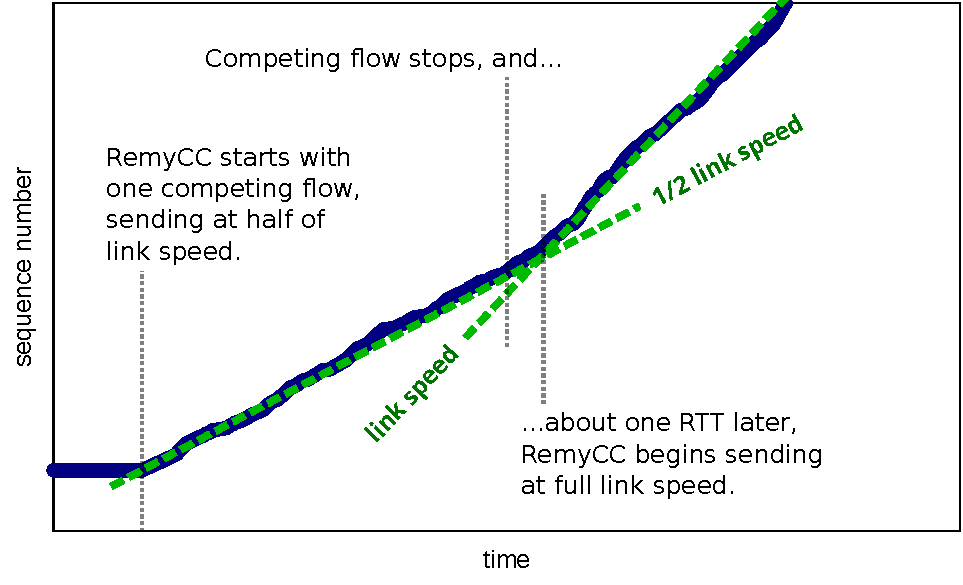
\includegraphics[width=\columnwidth]{trace.pdf}
\caption{Sequence plot of a RemyCC flow in contention with varying
  cross traffic. The flow responds quickly to the departure of a
  competing flow by doubling its sending rate.}
\label{f:trace}
\end{figure}

To explain this result, we investigated how multiple RemyCC flows
share the network. We found that when a new flow starts, the system
converges to an equitable allocation quickly, generally after little
more than one RTT. Figure~\ref{f:trace} shows the sequence of
transmissions of a new RemyCC flow that begins while sharing the link.
Midway through the flow, the competing traffic departs, allowing
the flow to start consuming the whole bottleneck rate.

\begin{figure}
%\vspace{\baselineskip}
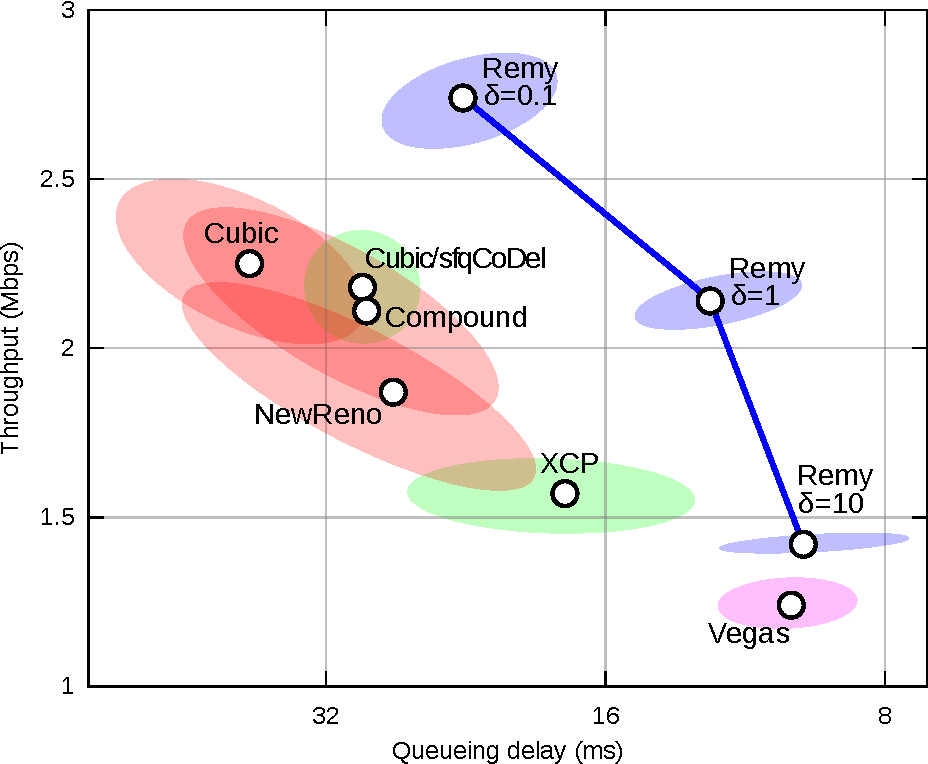
\includegraphics[width=\columnwidth]{vzw-4-final.pdf}
\caption{Verizon LTE downlink trace, $n = 4$. 1-$\sigma$ ellipses are shown.
The RemyCCs define the efficient frontier. Senders alternated between
exponentially-distributed file transfers (mean 100 kilobytes) and
exponentially-distributed pause times (mean 0.5 s).}
\label{f:verizon4}

\end{figure}

\begin{figure}
%\vspace{\baselineskip}
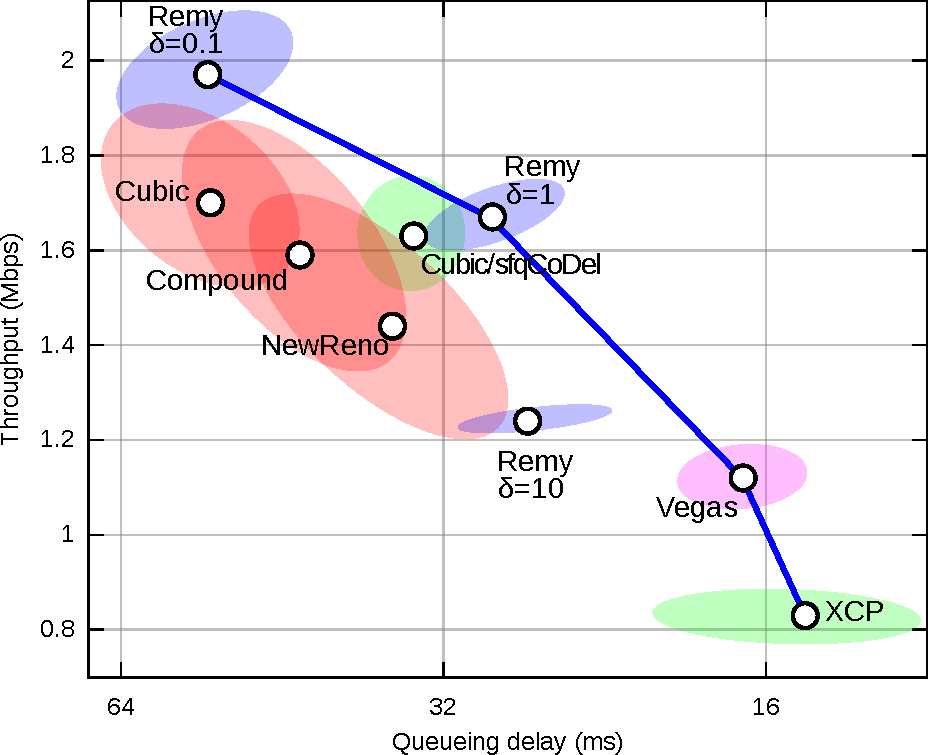
\includegraphics[width=\columnwidth]{vzw-8-final.pdf}
\caption{Verizon LTE downlink trace, $n = 8$. 1-$\sigma$ ellipses are
  shown.  As the degree of multiplexing increases, the schemes move
  closer together in performance and router-assisted schemes begin to
  perform better. Two of the three RemyCCs are on the efficient frontier.}
\label{f:verizon8}
\end{figure}

\begin{figure}
%\vspace{\baselineskip}
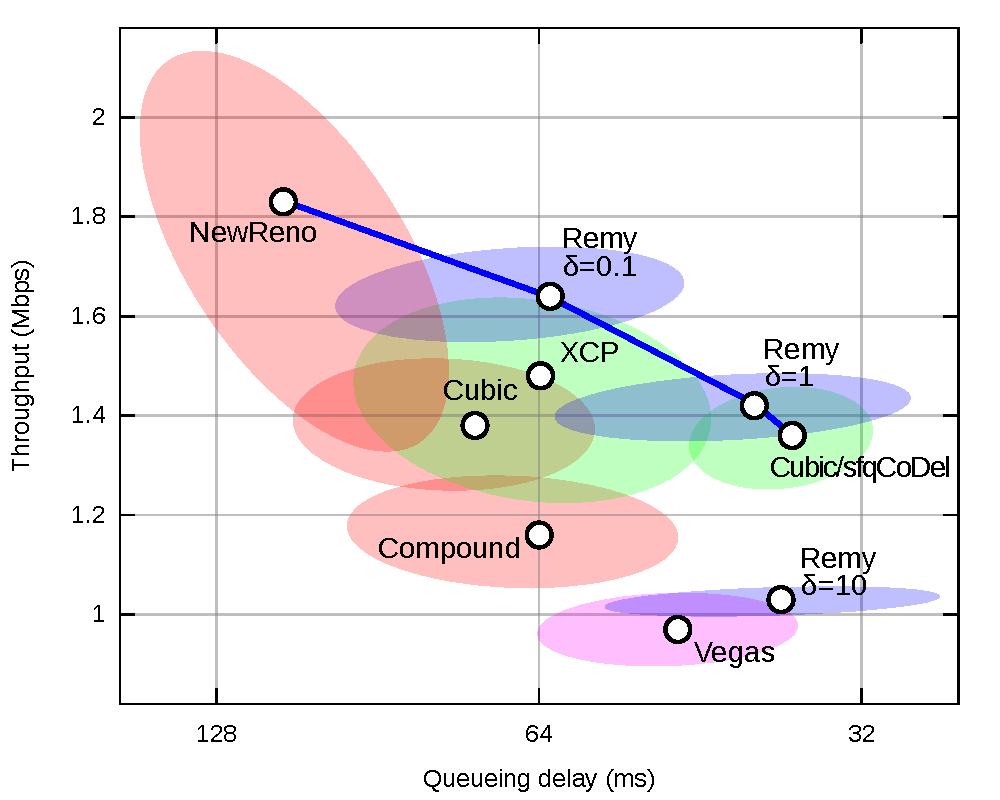
\includegraphics[width=\columnwidth]{att-4-final.pdf}
\caption{AT\&T LTE downlink trace, $n = 4$. Two of the RemyCCs are on
  the efficient frontier.}

\label{f:att2}
\end{figure}

%\pagebreak
\subsection{Cellular wireless links}

Cellular wireless links are tricky for congestion-control algorithms
because their link rates vary with time.\footnote{XCP, in particular,
  depends on knowing the speed of the link exactly; in our tests on cellular
  traces we supplied XCP with the long-term average link speed for
  this value.}

By running a program that attempts to keep a cellular link backlogged
but without causing buffer overflows, we measured the variation in
download speed on Verizon's and AT\&T's LTE service while mobile. We
then ran simulations over these pre-recorded traces, with the
assumption that packets are enqueued by the network until they can be
dequeued and delivered at the same instants seen in the trace.

%\begin{figure}
%\caption{Varying downlink capacity of the mobile Verizon LTE service
%  for a single user.}
%
%\label{f:celllinkvar}
%
%\vspace{\baselineskip}
%
%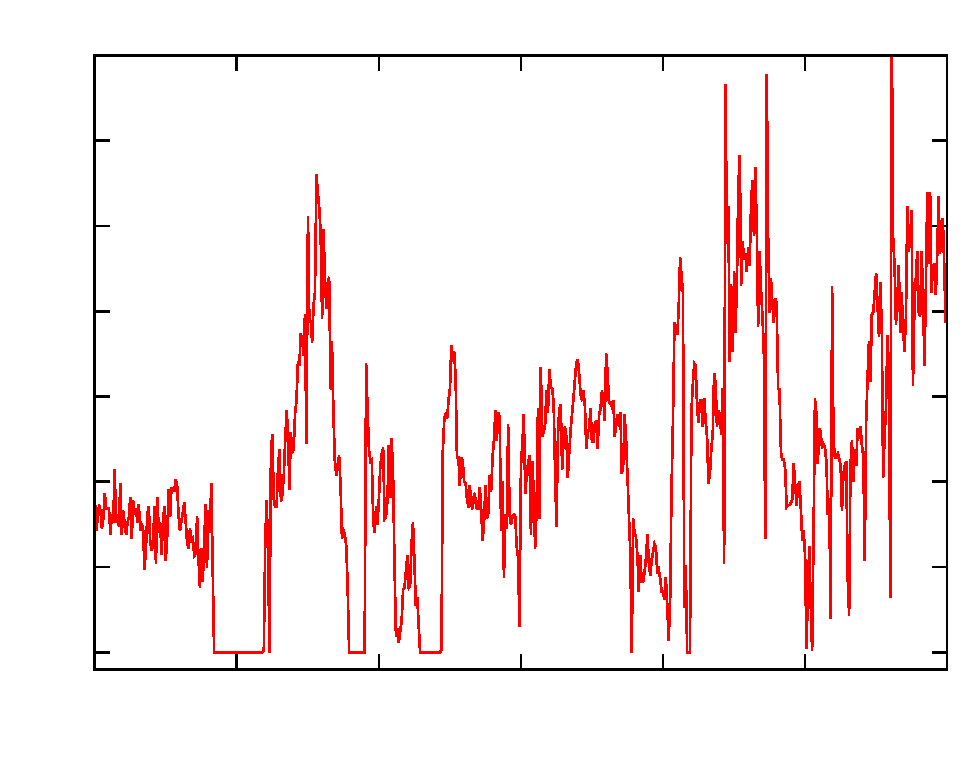
\includegraphics[width=\columnwidth]{verizon.pdf}
%
%\end{figure}

As discussed above, we did not design the RemyCCs to accommodate such a wide
variety of throughputs. Running the algorithm over this link
illustrated some of the limits of a RemyCC's generalizability beyond
situations encountered during the design phase.

Somewhat to our surprise, for moderate numbers of concurrent flows, $n
\le 8$, the RemyCCs continued to surpass (albeit narrowly) the best
human-designed algorithms, even ones benefiting from in-network
assistance. See Figures~\ref{f:verizon4} and \ref{f:verizon8}.

%However, for larger $n$, end-to-end RemyCCs no longer outperformed
%schemes with router participation. Figure~\ref{f:verizon32} shows the
%results of a simulation with $n = 32$ senders, all using the empirical
%distribution of flow lengths. The RemyCCs were no longer on the
%efficient frontier (the best schemes), although they did still
%outperform the human-designed end-to-end schemes except Vegas.

%Much further work will be necessary to assess the generalizability of
%a RemyCC. We discuss this in the next section.

%\begin{figure}
%\vspace{\baselineskip}
%\begin{centering}
%
%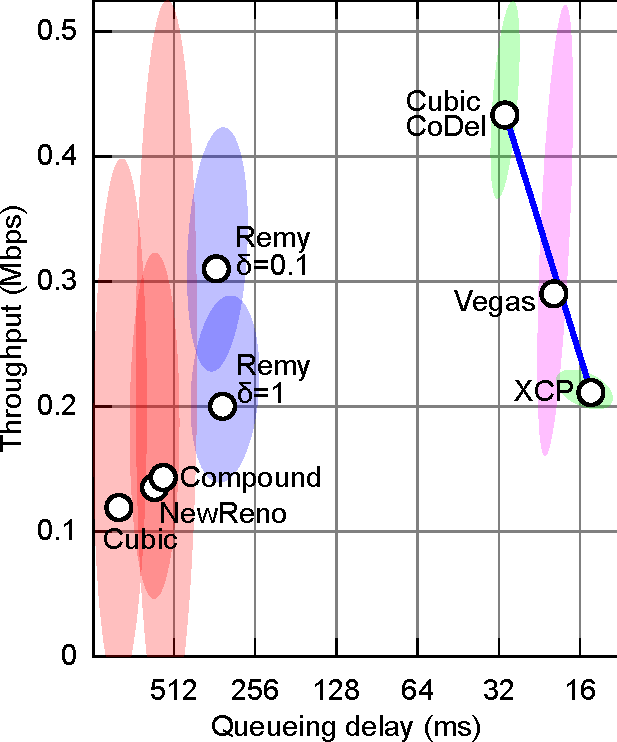
\includegraphics[width=.75\columnwidth]{verizon-32.pdf}
%
%\end{centering}

%\caption{When $n = 32$ on the Verizon trace, the RemyCCs are well
%  outside the limits of their design range of 1--16 senders. They outperform the
%  end-to-end congestion control methods except Vegas, but are beaten
%  by the in-network schemes.}

%\label{f:verizon32}
%
%\end{figure}

\subsection{Differing RTTs}

\begin{figure}
%\vspace{\baselineskip}

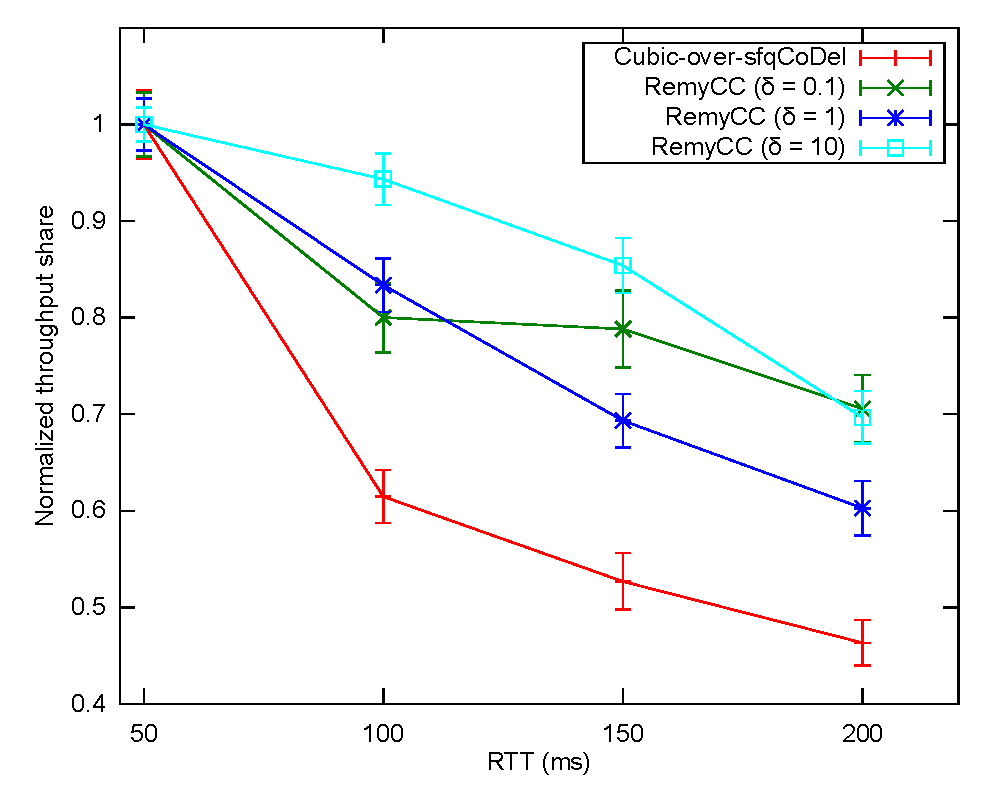
\includegraphics[width=\columnwidth]{rttfairness.pdf}
\caption{The RemyCCs' RTT unfairness compares favorably to
  Cubic-over-sfqCoDel. Error bar represents standard error of the mean
  over 128 100-second simulations.}

\label{f:fairness}

\end{figure}

We investigated how the RemyCCs allocate throughput on a contested
bottleneck link when the competing flows have different RTTs. At the
design stage, all contending flows had the same RTT (which was drawn
randomly for each network specimen from between 100~ms and 200~ms), so
the RemyCCs were not designed to exhibit RTT fairness explicitly.

We compared the RemyCCs with Cubic-over-sfqCoDel by running 128
realizations of a four-sender simulation where one sender-receiver
pair had RTT of 50~ms, one had 100~ms, one 150~ms, and one 200~ms. The
RemyCCs did exhibit RTT unfairness, but more modestly than
Cubic-over-sfqCoDel~(Fig.~\ref{f:fairness}).

\subsection{Datacenter-like topology}

We simulated 64 connections sharing a 10~Gbps datacenter link, and
compared DCTCP~\cite{dctcp} (using AQM inside the network) against
a RemyCC with a 1000-packet tail-drop queue. The RTT of
the path in the absence of queueing was 4 ms. Each sender sent 20
megabytes on average (exponentially distributed) with an ``off'' time
between its connections exponentially distributed with mean 100
milliseconds.

We used Remy to design a congestion-control algorithm to maximize
$-\frac{1}{\mbox{\footnotesize throughput}}$ (minimum potential delay) over these network
parameters, with the degree of multiplexing assumed to have been drawn
uniformly between 1 and 64.

%To do this, we simple speeded up the internal timebase of the RemyCC
%by a thousandfold. Its action variable $r$ was interpreted as a number
%of microseconds instead of milliseconds, etc. The design range of
%10--20 Mbps became a design range of 10--20 Gbps, still an order of
%magnitude away from the actual link speed.

%We compared this RemyCC with DCTCP~\cite{dctcp}, a well-known protocol
%tuned for datacenters with high bandwidths and low propagation delays
%that runs at endpoints and also inside the network.

% We found that the median DCTCP throughput averaged over 2,048
% connections was 141 Mbps, compared with 305 Mbps for the
% RemyCC. Although Remy came close to matching the human-designed
% in-network scheme, it did not outperform it in this data-center-like
% application. 

The results for the mean and median throughput (tput) for the 20 megabyte
transfers are shown in the following table:

\begin{tabular}{lll}
& \bf tput: mean, med & \bf rtt: mean, med\\
%   & ~~(Mbps) & ~~(ms)\\
\bf DCTCP (ECN) & 179, 144 Mbps & 7.5, 6.4 ms\\
\bf RemyCC (DropTail) & 175, 158 Mbps & 34, 39 ms \\
%\bf RemyCC+RED & 102,  & \\
\vspace{\baselineskip}
\end{tabular}

These results show that a RemyCC trained for the datacenter-network
parameter range achieves comparable throughput at lower variance than
DCTCP, a published and deployed protocol for similar scenarios. The
per-packet latencies (and loss rates, not shown) are higher, because
in this experiment RemyCC operates over a DropTail bottleneck router,
whereas DCTCP runs over an ECN-enabled RED gateway that marks packets
when the instantaneous queue exceeds a certain threshold. Developing
RemyCC schemes for networks with ECN and AQM is an area for future
work.

\begin{comment}
\subsection{Competing protocols}

We investigated the possibility of incremental deployment of a RemyCC,
by simulating a single bottleneck link with one RemyCC flow contending
with one flow from either Compound or Cubic, with no active queue
management. The RemyCC was designed for round-trip-times between
100~ms and 10~s, in order to accommodate a ``buffer-filling''
competitor on the same bottleneck link.

We used the same observed traffic distribution from
Figure~\ref{f:flowcdf} and varied the mean ``off'' time (exponentially
distributed) of the senders.  The bottleneck link speed was 15~Mbps
and baseline RTT was 150 ms. We also experimented with flows of mean
sizes 100 kilobytes and 1 megabyte, with an exponentially distributed mean
``off'' time of 0.5 seconds between successive flows. 

The results, shown in the two tables below, depended on the duty cycle
of the senders dictated by the mean off time (numbers in parentheses
are standard deviations).

\vspace{\baselineskip}

% \begin{tabular}{lll}
% \bf Mean off time & \bf RemyCC tput & \bf Compound tput \\
% \hline 0.2~sec & 3.8~Mbps & 3.0~Mbps \\
% 0.1 & 4.1 & 4.4 \\
% 0.01 & 0.84 & 9.2 \\
% \end{tabular}

\begin{tabular}{lll}
\bf Mean off time & \bf RemyCC tput & \bf Compound tput \\
\hline 200 ms & 2.12 (.11)~Mbps & 1.79 (.18)~Mbps \\
100 & 2.18 (.08)  & 2.75 (.27)\\
10 & 2.28 (.10) & 3.9 (.13) \\
\hline
\bf Mean size & \bf RemyCC tput & \bf Cubic tput \\
100 KBytes & 2.04 (.14) & 1.31 (.16)\\
1 MByte & 2.09 (.11) & 1.28 (.11) \\
\hline
\end{tabular}

\vspace{\baselineskip}

% \begin{tabular}{lll}
% \bf Mean off time & \bf RemyCC tput & \bf Cubic tput \\
% \hline 0.2~sec & 3.4~Mbps & 3.2~Mbps \\
% 0.1 & 2.3 & 6.1 \\
% 0.01 & 0.74 & 9.3 \\
% \end{tabular}

%0.01 & 2.32 (0.1) & 3.95 (.16)  \\
%\bf Mean size & \bf RemyCC tput & \bf Cubic tput \\
%\hline
%100 KBytes & 2.06 (.13) & 1.23 (.12)\\
%1 MByte & 2.07 (.13) & 1.27 (.09) \\
%\hline
%\end{tabular}

%\vspace{\baselineskip}

We observe that this RemyCC does well at low duty cycles because it is
able to grab spare bandwidth more quickly. At higher duty cycles (with
low mean off time), Cubic and Compound tend to grab a higher share of
the bandwidth. The results, however, are close enough that we believe
a RemyCC designed for competing with more aggressive protocols may
close the gap, while retaining high performance when competing only with
like-minded RemyCCs.

\subsection{How helpful is prior knowledge about the network?}

We investigated the performance benefit conferred by having
more-specific prior information about the network, and what happens
when that prior information is incorrect.

We used Remy to construct two additional RemyCCs, each for a network
with a known minimum RTT of 150~ms. For one RemyCC, the link speed was
assumed to be 15~Mbps exactly. A second RemyCC was designed to span
a 10$\times$ range of link speeds, from 4.7~Mbps to 47~Mbps. We also
compared against Cubic-over-sfqCoDel over this range.

The results are shown in Figure~\ref{f:spec}. On the particular link
for which the ``1$\times$'' RemyCC was designed, it performs the best,
but its performance trails off quickly around that value. Within the
range of the ``10$\times$'' RemyCC, it beats Cubic-over-sfqCoDel, but
again deteriorates when the true network violates its design
assumptions. The results show that more-specific prior knowledge is
helpful and improves performance --- when it happens to be correct.

\begin{figure}
%\vspace{\baselineskip}
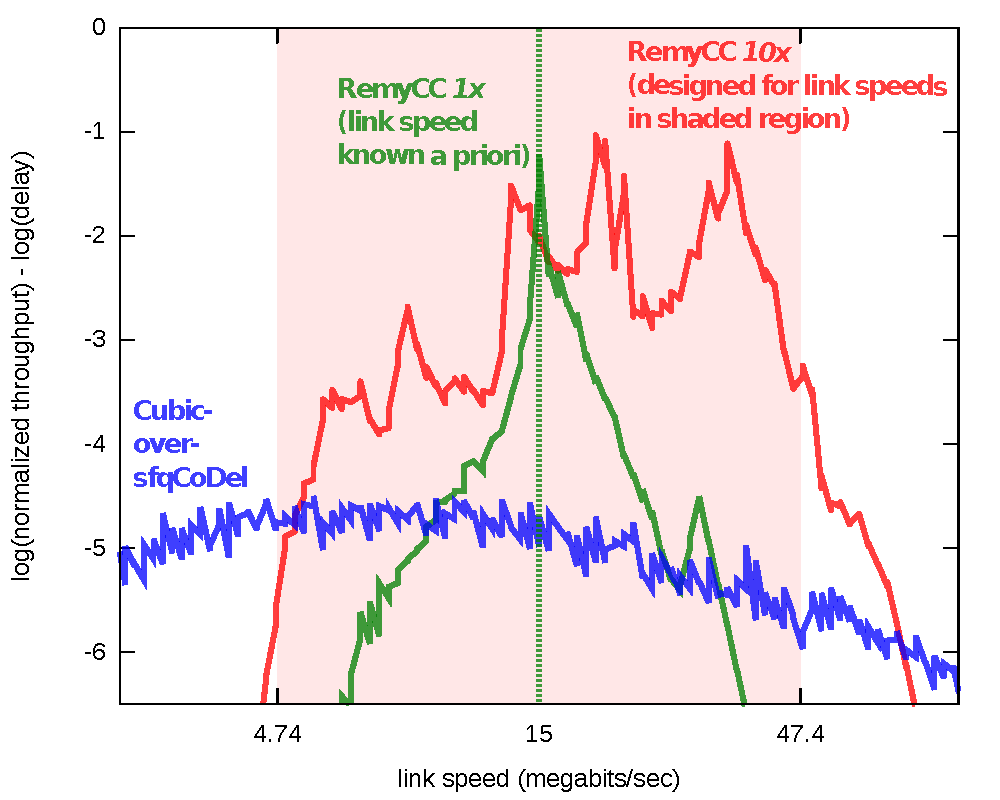
\includegraphics[width=\columnwidth]{spec2.pdf}
\caption{Performance of two end-to-end RemyCCs that were designed with
  different prior information about the network, compared with
  Cubic-over-sfqCoDel as the link speed varies. Despite running only
  at the sender, the RemyCCs each outperform Cubic-over-sfqCoDel over
  almost their entire design ranges. But when a RemyCC's
  assumptions aren't met, performance deteriorates.}

\label{f:spec}

\end{figure}

\subsection{Summary of results}

Using a few CPU-weeks of computation,
Remy produced several computer-generated congestion-control algorithms,
which we then evaluated on a variety of simulated network conditions
of varying similarity to the prior assumptions supplied at design-time.

On networks whose parameters mostly obeyed the prior knowledge
supplied at design range --- such as the dumbbell network with the
15~Mbps link --- Remy's end-to-end algorithms outperformed all of the
human-generated congestion-control algorithms, even algorithms that
receive help from network infrastructure.

RemyCC ($\delta = 0.1)$ achieved $> 1.7\times$ gains in median
throughput and $> 2.7\times$ reductions in median queueing delay
against Cubic and Compound, generally thought to be excellent
general-purpose congestion-control algorithms. Against
Cubic-over-sfqCoDel, which has the benefit of code running on network
infrastructure, RemyCC achieved a 40\% increase in median throughput
and a $7.8\times$ decrease in median queueing delay.

On the cellular link traces, which are variable and were not designed
for, Remy's schemes outperformed the existing congestion-control
algorithms (end-to-end or otherwise) when the maximum degree of
multiplexing was 4 or less, and outperformed the end-to-end schemes
and sfqCoDel when it was 8 or less. However, as the network conditions
grew farther afield from the supplied prior assumptions, Remy's
performance declined, although the algorithms were still competitive
with traditional TCP congestion control on the networks we examined.

\end{comment}
